\section{Two Task Result}

We will first consider the simplest case, where there are only two tasks: one producing a value and one consuming it. By considering just the first task $A$ we can see that the worst case is shown in Figure 1. Note that this scenario assumes schedulability to ensure that one job of $A$ must run and complete within each period. This is where our assumption of schedulability becomes vital for our correct solution.

\begin{figure}[!ht]
	\centering
	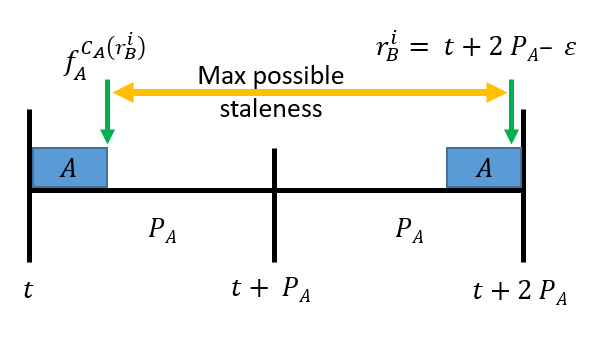
\includegraphics[width=2.5in]{figures/2TaskMaxStaleness}
	\caption{Maximum Staleness Scenario for Data from Task A.}
	\label{fig:2Tasks}
\end{figure}

Figure \ref{fig:2Tasks} labels the maximum separation between the publishing of output data from the depicted task. In order to maximize the staleness, we assume the reading task, task B, is released arbitrarily close, but before, the finish of the second job of task A. If we take push the second task towards the end of its period we see that the maximum staleness is when the second job finishes at the instant its period ends.

\begin{theorem}
	\label{thm:2TaskMaxWaiting}
	The scenario in Figure \ref{fig:2Tasks}, i.e., when a job is executed and completed at the very beginning of a period and the next job completes at the very end of the next period, is the upper bound scenario for data freshness, as defined in Section III, produced by that task.
\end{theorem}

\begin{proof}
	First note that one job must be executed within each period, as per definition of periodic tasks and our assumption that the task set is schedulable.
	
	Consider any placement of two jobs of a task within two consecutive periods. Assume this instance is not the instance depicted in Figure \ref{fig:2Tasks}. Then at least one of the following apply:
	\begin{case}
		The job in the first period is not completed as soon as possible. In this case, move when this task first starts execution $\epsilon$ earlier. This increases the staleness by $\epsilon$ and moves the job's finishing time towards the tasks execution time after that period.
	\end{case}
	\begin{case}
		The job in the second period is not completed as late as possible. In this case, move when this task first starts execution $\epsilon$ later. This increases the staleness by $\epsilon$ and moves the job's finishing time close to the end of the period.
	\end{case}
	Since all instantiations of the problem can be moved closer to the depicted instance while strictly increasing the staleness, it holds that this instance is the unique worst case for staleness.
\end{proof}

Now that we have proved the above scenario is the worst case with regards to the freshness of data from task $A$, we can use algebra to solve for the constraint on $P_A$. From Figure \ref{fig:2Tasks}, we can see that the maximum staleness is composed of two periods of $A$ less one execution time of $A$ less $\epsilon$, and we want this to be less than our freshness bound $d_{A \to B}$, i.e. $d_{A \to B} \geq 2P_A-E^l_A-\epsilon$. We can then solve for $P_A$ to prove the following lemma.

Note that we assume the best case execution time for the first task in order to stretch the freshness as long as possible. If we assume that the first task in a two task scenario executes at its worst case, then $E^l_A$ in our solution will be replaced with $E^u_A$.

\begin{lemma}
	\label{lem:2TaskResult}
	To ensure the output of task $A$ is always at most $d_{A \to B}$ old, choose $P_A \leq \frac{d_{A \to B} + E^l_A}{2}$.
\end{lemma}

\begin{proof}
	\begin{align*}
		d_{A \to B}&\geq 2P_A-E^l_A-\epsilon &\mbox{From Figure \ref{fig:2Tasks}}&\\
		d_{A \to B}&\geq 2P_A-E^l_A &\mbox{$\epsilon \to 0$}&\\
		2P_A&\leq d_{A \to B} + E^l_A &\mbox{Add $E_A$, swap sides}&\\
		P_A&\leq \frac{d_{A \to B} + E^l_A}{2} &\mbox{Divide by 2}&\\
	\end{align*}
\end{proof}

Thus we see that if we set $P_A$ to the the above quantity we ensure that the output of task $A$ is always at most $d_{A \to B}$ old, and therefore can only ever be at most this old when consumed by task $B$. Since $P_A$ is the only parameter under our control, we can also set it less than this quantity and maintain the freshness guarantee (this would in essence force $d_{A \to B}$ smaller, and a smaller freshness guarantee will always ensure a larger one as well).

Recall that our fitness metric is total utilization. Since the parameters of $B$ are irrelevant in the solution and $E_A$ is fixed, our only optimization parameter is $P_A$. It is trivial to see that choosing $P_A$ as large as possible will minimize the task set utilization, and thus the above, when set equal to the right-hand quantity, is the solution for the two task scenario while optimizing over task set utilization. Note that this value may not produce a schedulable task set. If this is the case, the largest schedulable period that meets the above inequality is the solution. Note that for many systems decreasing $P_A$ can only worsen schedulability. For these systems, if the task set is unschedulable when set equal to the above quantity then there does not exist any $P_A$ for which the freshness guarantee is met with a schedulable task set.
